\section{FPGA}

\begin{frame}{\textbf{FPGA简介}}
\phantomsection\label{fpga}
\begin{itemize}
\tightlist
\item
    \textbf{市场背景}:

    \begin{itemize}
    \tightlist
    \item
    FPGA
    市场是半导体行业中增长最快的领域之一,但其市场格局变化迅速,公司在其中的参与度也在快速变化。
    \item
    由于很难预测行业稳定时哪些产品将成为主流,因此本节将聚焦于当前广泛使用的产品,而非列举所有
    FPGA 制造商。
    \end{itemize}
\item
    \textbf{容量描述}:

    \begin{itemize}
    \tightlist
    \item
    在描述每个器件时,将列出其容量,通常以供应商提供的等效 2
    输入与非门(NAND 门)数量表示。
    \item
    注意:FPGA 行业中的门数计算存在争议,因此本文提供的数字仅供参考。
    \end{itemize}
\item
    \textbf{FPGA 分类}:

    \begin{enumerate}
    \tightlist
    \item
    \textbf{基于 SRAM 的 FPGA}:

    \begin{itemize}
    \tightlist
    \item
        主要厂商:Xilinx 和 Altera,AT\&T 是主要竞争对手。
    \end{itemize}
    \item
    \textbf{基于反熔丝的 FPGA}:

    \begin{itemize}
    \tightlist
    \item
        主要厂商:Actel、Quicklogic、Cypress 和 Xilinx。
    \end{itemize}
    \end{enumerate}
\end{itemize}
\end{frame}

\subsection{Xilinx FPGA}
\begin{frame}{\textbf{Xilinx基于SRAM的FPGA的基本结构}}
\begin{figure}
    \centering
    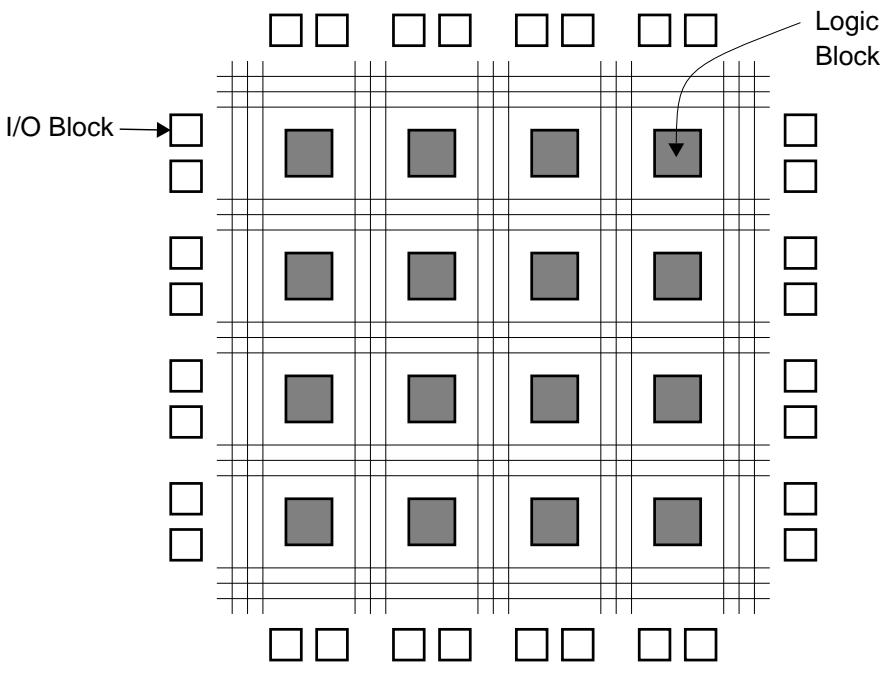
\includegraphics[width=0.5\textwidth]{img1/FPGA.jpeg}
    \caption{Xilinx FPGA 的基本结构}
\end{figure}
    Xilinx FPGA
    的基本结构是\textbf{基于阵列的},即每个芯片由一个二维逻辑块阵列组成,逻辑块通过水平和垂直的布线通道互连。
\end{frame}

\begin{frame}{Xilinx FPGA产品系列}:
\begin{itemize}
\item
    \textbf{XC2000 系列}: 首个 FPGA 系列,于1985年推出。
\item
    \textbf{XC3000 系列}: 仍广泛使用。
\item
    \textbf{XC4000 系列}: 更现代且更受欢迎的系列。
\item
    \textbf{XC5000 系列}: 与 XC4000
    类似,但以更具吸引力的价格提供相似功能,速度略有损失。
\item
    \textbf{XC8100 系列}: 基于反熔丝技术的新系列,暂未广泛使用。
\item
    \textbf{容量范围}: XC4000 系列的容量从约 2000 到超过 15000 等效门。
\end{itemize}
\end{frame}

\begin{frame}[allowframebreaks]{\textbf{XC4000 逻辑块(CLB)}:}
\begin{itemize}
\tightlist
\item
    \textbf{查找表(LUTs)}:

    \begin{itemize}
    \tightlist
    \item
    LUT 是一个小型的单比特宽存储阵列,存储器地址线是逻辑块的输入,输出是
    LUT 的输出。
    \item
    一个具有 K 个输入的 LUT 对应一个 2\^{}K x 1
    比特的存储器,通过将逻辑函数的真值表编程到存储器中,可以实现任意 K
    输入逻辑函数。
    \end{itemize}
\item
    \textbf{CLB 结构}:

    \begin{itemize}
    \tightlist
    \item
    如图18所示,每个 CLB 包含三个独立的 LUT:

    \begin{itemize}
    \tightlist
    \item
        两个 4 输入 LUT,由 CLB 输入驱动。
    \item
        第三个 LUT 可以与前两个结合使用。
    \end{itemize}
    \item
    这种配置允许 CLB 实现多达 9 输入的广泛逻辑函数,或实现两个独立的 4
    输入函数。
    \item
    每个 CLB 还包含两个触发器。
    \end{itemize}
\end{itemize}

\begin{figure}
    \centering
    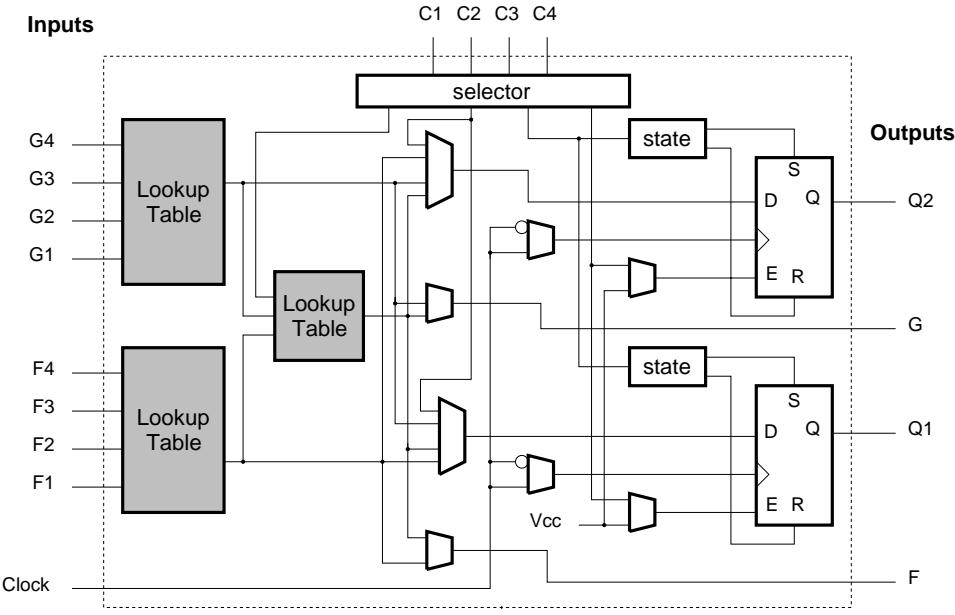
\includegraphics[width=0.6\textwidth]{img1/XC4000.jpeg}
    \caption{Xilinx XC4000 可配置逻辑块(CLB)}
\end{figure}

\end{frame}

\begin{frame}{\textbf{系统级特性}:}
\phantomsection\label{ux7cfbux7edfux7ea7ux7279ux6027}
\begin{itemize}
\tightlist
\item
    \textbf{算术电路}: 每个 CLB
    包含高效执行算术运算的电路(如快速进位操作)。
\item
    \textbf{RAM 配置}: CLB 中的 LUT 可以配置为读/写 RAM 单元。
\item
    \textbf{XC4000E 版本}:

    \begin{itemize}
    \tightlist
    \item
    RAM 可以配置为双端口 RAM,具有一个写端口和两个读端口。
    \item
    RAM 块可以配置为同步 RAM。
    \end{itemize}
\item
    \textbf{宽与门平面}:
    芯片外围包含非常宽的与门平面,便于实现宽解码器等电路块。
\end{itemize}
\end{frame}

\begin{frame}[allowframebreaks]{\textbf{互连结构}:}
\begin{itemize}
\tightlist
\item
    互连结构是 FPGA 的另一个关键特征。
\item
    \textbf{布线通道}:

    \begin{itemize}
    \tightlist
    \item
    分为水平和垂直通道。
    \item
    通道中包含:

    \begin{itemize}
    \tightlist
    \item
        短线段:跨越单个 CLB。
    \item
        长线段:跨越两个 CLB。
    \item
        超长线段:跨越整个芯片的长度或宽度。
    \end{itemize}
    \item
    可编程开关用于连接 CLB 的输入输出和线段,或连接不同的线段。
    \end{itemize}
\item
    \textbf{重要特点}:

    \begin{itemize}
    \tightlist
    \item
    信号必须通过开关从一个 CLB 传递到另一个
    CLB,所经过的开关数量取决于所使用的线段。
    \item
    因此,实现电路的速度性能部分取决于 CAD 工具如何分配线段给各个信号。
    \end{itemize}
\end{itemize}

\begin{figure}
    \centering
    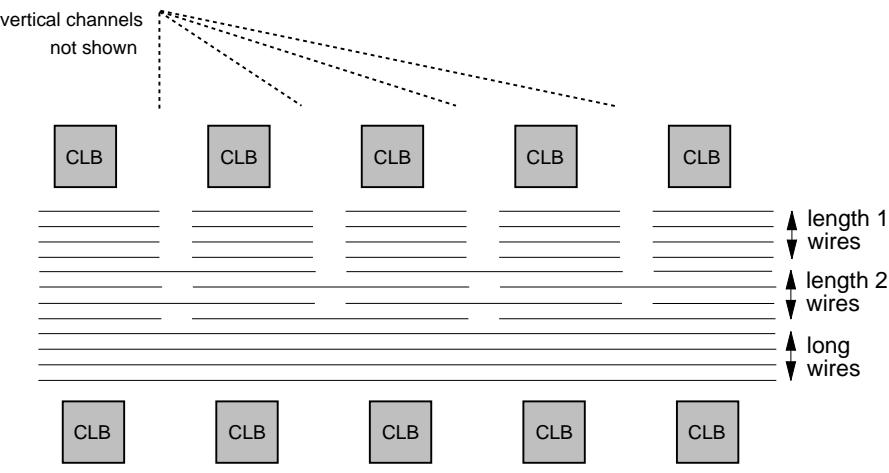
\includegraphics[width=0.6\textwidth,keepaspectratio]{img1/XC4000Wire.jpeg}
    \caption{Xilinx XC4000 线段示意图。}
\end{figure}

\end{frame}

\begin{frame}[allowframebreaks]{\textbf{Xilinx Artix-7 XC7A35T FPGA 的结构}}
\begin{itemize}
\tightlist
\item
    Xilinx Artix-7 XC7A35T FPGA 主要由以下九个组件构成:

    \begin{enumerate}
    \tightlist
    \item
    输入/输出块(I/O Blocks)
    \item
    可配置逻辑块(CLBs)
    \item
    互连资源
    \item
    块 RAM
    \item
    DSP 切片
    \item
    时钟管理块
    \item
    XADC 块
    \item
    高速串行 I/O 收发器
    \item
    PCIe 接口
    \end{enumerate}
\item
    大多数模块也可以通过 Vivado 设计套件观察到。
\item
    这些模块(或其变体)在 FPGA 中几乎是标准的,但不同 FPGA
    家族可能会缺少某些模块或包含额外的模块。
\end{itemize}

\begin{figure}
    \centering
    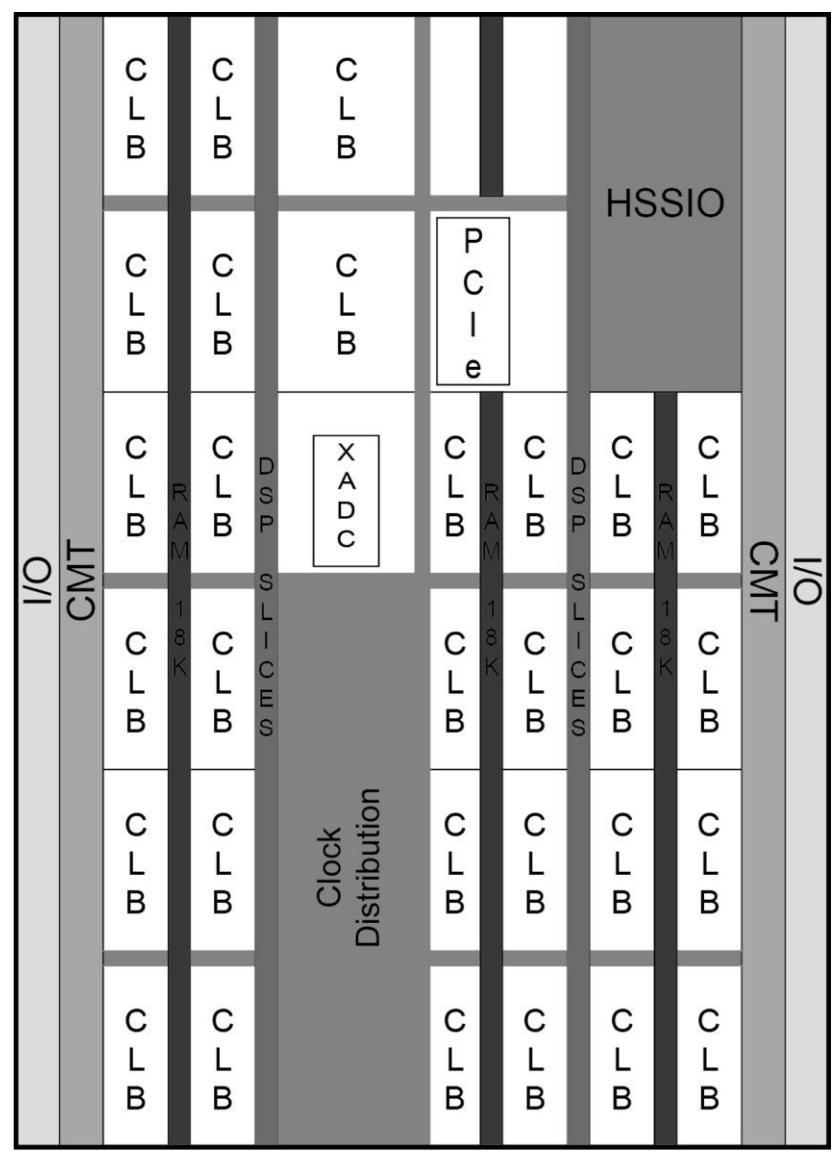
\includegraphics[width=0.4\textwidth,keepaspectratio]{img1/XC7A35T.jpeg}
    \caption{Artix-7 XC7A35T FPGA 的基本组成模块。}
\end{figure}

\end{frame}

\begin{frame}[allowframebreaks]{\textbf{输入/输出块}}
\begin{block}{\textbf{简介}}
\phantomsection\label{ux7b80ux4ecb}
\begin{itemize}
\tightlist
\item
    数字设备通过其输入和输出引脚与外界交互,FPGA 也不例外。
\item
    数据通过输入引脚从外部获取,输出引脚用于将数据输出到外部。
\item
    这些输入和输出引脚位于 FPGA 的输入/输出块中。
\end{itemize}
\end{block}

\begin{block}{\textbf{电压与引脚数量}}
\phantomsection\label{ux7535ux538bux4e0eux5f15ux811aux6570ux91cf}
\begin{itemize}
\tightlist
\item
    Artix-7 XC7A35T FPGA 的输入/输出引脚支持标准电压范围:1.2 到 3.3 V。
\item
    Basys3 开发板上的 FPGA 有 106 个输入/输出引脚。
\item
    Arty 开发板上的 FPGA 有 210 个输入/输出引脚。
\item
    这些引脚可以用作输入、输出或两者兼用。
\end{itemize}
\end{block}

\begin{block}{\textbf{引脚模式}}
\phantomsection\label{ux5f15ux811aux6a21ux5f0f}
\begin{enumerate}
\tightlist
\item
    \textbf{输入模式}: 通过引脚从外部获取数据。
\item
    \textbf{输出模式}: 通过引脚向外部输出电压电平。
\item
    \textbf{双向模式}: 同一引脚可用于输入和输出。
\end{enumerate}
\end{block}

\begin{block}{\textbf{引脚分组与模式}}
\phantomsection\label{ux5f15ux811aux5206ux7ec4ux4e0eux6a21ux5f0f}
\begin{itemize}
\tightlist
\item
    输入/输出引脚被分组为\textbf{组(Banks)}。
\item
    每组中的两个引脚被分组为正(P)负(N)对。
\item
    \textbf{单端模式}:

    \begin{itemize}
    \tightlist
    \item
    输入电压接近地电平时,逻辑电平为 0。
    \item
    输入电压接近 \emph{VCC} 时,逻辑电平为 1。
    \end{itemize}
\item
    \textbf{差分模式}:

    \begin{itemize}
    \tightlist
    \item
    引脚 P 的电压低于引脚 N 时,逻辑电平为 0。
    \item
    引脚 P 的电压高于引脚 N 时,逻辑电平为 1。
    \end{itemize}
\item
    \textbf{参考模式}:

    \begin{itemize}
    \tightlist
    \item
    输入电压低于参考电压时,逻辑电平为 0。
    \item
    输入电压高于参考电压时,逻辑电平为 1。
    \end{itemize}
\end{itemize}
\end{block}

\begin{block}{\textbf{输出模式}}
\phantomsection\label{ux8f93ux51faux6a21ux5f0f}
\begin{itemize}
\tightlist
\item
    单端引脚也可用作输出。

    \begin{itemize}
    \tightlist
    \item
    逻辑电平为 1 时,引脚电压为 \emph{VCC}。
    \item
    逻辑电平为 0 时,引脚电压为地电平。
    \end{itemize}
\end{itemize}
\end{block}
\end{frame}

\begin{frame}[allowframebreaks]{\textbf{可配置逻辑块(CLB)}}
\begin{itemize}
\tightlist
\item
    \textbf{简介}:

    \begin{itemize}
    \tightlist
    \item
    可配置逻辑块(CLB)是 FPGA 中实现数字系统的基本元素。
    \item
    CLB 的核心包括查找表(LUT)、触发器和多路复用器。
    \end{itemize}
\end{itemize}

\begin{block}{\textbf{多路复用器}}
\phantomsection\label{ux591aux8defux590dux7528ux5668}
\begin{itemize}
\tightlist
\item
    \textbf{基本概念}:

    \begin{itemize}
    \tightlist
    \item
    多路复用器是一种选择器,具有 \emph{N} 个选择位、2 \emph{N}
    个输入引脚和1个输出引脚。
    \item
    通过选择位决定哪个输入引脚连接到输出。
    \end{itemize}
\item
    \textbf{二选一多路复用器}:

    \begin{itemize}
    \tightlist
    \item
    图2.10展示了由基本逻辑门构成的二选一多路复用器的电路图。
    \item
    工作原理:
    \[out = \begin{cases} \text{in1} & \text{if sel = 0} \\ \text{in2} & \text{if sel = 1} \end{cases} \tag{2.4}\]
    \item
    选择引脚(sel)决定哪个输入连接到输出。
    \end{itemize}
\item
    \textbf{32选1多路复用器}:

    \begin{itemize}
    \tightlist
    \item
    有5个选择位,可以选择32个输入中的其中一个。
    \end{itemize}
\end{itemize}

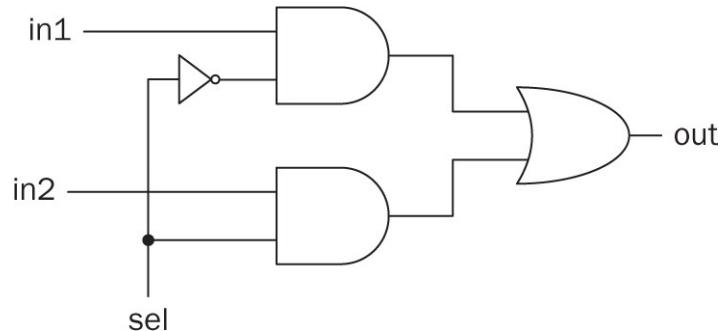
\includegraphics[keepaspectratio]{img1/XC7A35TMUX.jpeg}\\
\textbf{图13 - 由基本逻辑门构成的二选一多路复用器电路图。}
\end{block}

\begin{block}{\textbf{触发器}}
\begin{itemize}
\tightlist
\item
    \textbf{基本概念}:

    \begin{itemize}
    \tightlist
    \item
    触发器是 FPGA 中的基本存储单元,能够存储1位数据。
    \item
    触发器可以通过数字逻辑门构建,但其布局较为复杂。
    \item
    触发器只能存储逻辑电平0或1。
    \end{itemize}
\end{itemize}

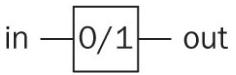
\includegraphics[keepaspectratio]{img1/XC7A35TFF.jpeg}\\
\textbf{图14 - 触发器的抽象表示。}
\end{block}

\begin{block}{\textbf{查找表(LUT)}}
\phantomsection\label{ux67e5ux627eux8868lut}
\begin{itemize}
\tightlist
\item
    \textbf{基本概念}:

    \begin{itemize}
    \tightlist
    \item
    LUT 是一组触发器,连接到多路复用器的输入引脚。
    \item
    多路复用器的选择位用于选择要访问的触发器地址。
    \item
    LUT 可以实现任何以选择位为输入变量的组合逻辑函数。
    \item
    当触发器的内容改变时,实现的逻辑函数也会改变,从而实现 FPGA
    的可重构性。
    \end{itemize}
\item
    \textbf{N 输入 LUT}:

    \begin{itemize}
    \tightlist
    \item
    具有 2 \emph{N} 个表项,\emph{N} 个选择位。
    \item
    图2.12展示了一个由触发器和多路复用器构成的抽象 LUT。
    \item
    Artix-7 FPGA 中,两个5输入的 LUT
    可以组合实现6输入、7输入或8输入的组合逻辑函数。
    \end{itemize}
\end{itemize}

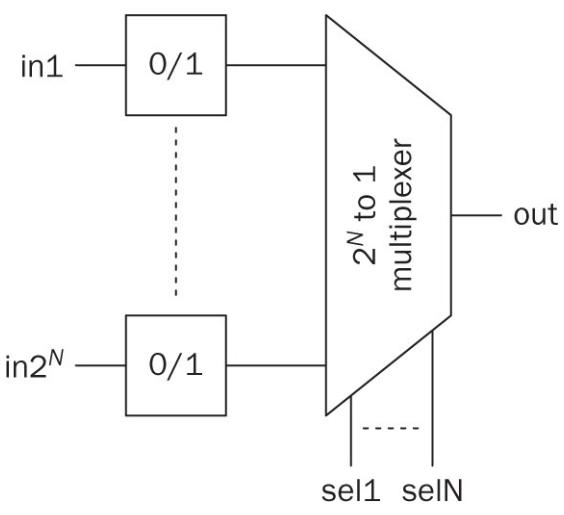
\includegraphics[keepaspectratio]{img1/XC7A35LUT.jpeg}\\
\textbf{图14 - N 输入 LUT 的抽象表示。}
\end{block}
\end{frame}

\begin{frame}{\textbf{互连资源}}
\phantomsection\label{ux4e92ux8fdeux8d44ux6e90}
\begin{itemize}
\tightlist
\item
    \textbf{简介}:

    \begin{itemize}
    \tightlist
    \item
    互连资源由电线和可编程开关组成,负责连接 FPGA 中的 CLB
    和其他构建模块。
    \item
    互连也称为布线通道。
    \item
    Artix-7 FPGA 中的 CLB 以网格结构布置,简化了互连使用的规划。
    \item
    初级或中级用户无需了解互连功能,Vivado
    设计套件负责高效使用这些资源。
    \end{itemize}
\end{itemize}
\end{frame}

\begin{frame}{\textbf{块 RAM}}
\phantomsection\label{ux5757-ram}
\begin{itemize}
\tightlist
\item
    \textbf{简介}:

    \begin{itemize}
    \tightlist
    \item
    与由 SLICEM 块组成的分布式存储元件不同,Artix-7 FPGA 还具有块 RAM
    模块。
    \item
    块 RAM 可用于存储数据,还可以构成缓冲区、大型 LUT 或移位寄存器。
    \end{itemize}
\item
    \textbf{容量}:

    \begin{itemize}
    \tightlist
    \item
    每个块 RAM 可以存储 36-kbit 的数据块或两个 18-kbit 的数据块。
    \item
    FPGA 中共有 50 个块 RAM,总容量为 1800 kbits。
    \item
    每个 36-kbit 块 RAM 的数据宽度为 64 位,额外 8
    位用于数据读取过程中的单比特错误纠正或双比特错误检测。
    \end{itemize}
\end{itemize}
\end{frame}

\begin{frame}{\textbf{DSP 切片}}
\phantomsection\label{dsp-ux5207ux7247}
\begin{itemize}
\tightlist
\item
    \textbf{简介}:

    \begin{itemize}
    \tightlist
    \item
    现代 FPGA
    中有专门用于算术和逻辑运算的模块,称为数字信号处理(DSP)切片。
    \item
    Artix-7 FPGA 中的 DSP 切片称为 DSP48E1,共有 90 个。
    \end{itemize}
\item
    \textbf{功能}:

    \begin{itemize}
    \tightlist
    \item
    每个 DSP 切片可以执行多种算术和逻辑运算,包括:

    \begin{itemize}
    \tightlist
    \item
        25 位和 18 位二进制数的乘法。
    \item
        48 位数的加法、减法和累加。
    \item
        48 位数的逻辑运算。
    \end{itemize}
    \item
    这些运算在没有 DSP 切片的情况下需要复杂的算法实现,因此 DSP
    切片在实现中非常高效。
    \end{itemize}
\end{itemize}
\end{frame}

\begin{frame}{\textbf{时钟管理}}
\phantomsection\label{ux65f6ux949fux7ba1ux7406}
\begin{itemize}
\tightlist
\item
    \textbf{简介}:

    \begin{itemize}
    \tightlist
    \item
    时钟是一个周期性方波信号,用于同步数字系统的运行。
    \item
    大多数数字系统需要时钟信号来同步逻辑操作。
    \end{itemize}
\item
    \textbf{时钟管理}:

    \begin{itemize}
    \tightlist
    \item
    Artix-7 FPGA 没有内部时钟生成电路,用户需要向 FPGA 提供时钟信号。
    \item
    一些输入/输出引脚能够接收时钟信号。
    \item
    时钟信号进入 FPGA 后,可以由时钟管理模块(CMT)处理并分配到整个
    FPGA。
    \item
    Basys3 和 Arty 开发板提供外部时钟源。
    \item
    Artix-7 FPGA 分为六个时钟区域,每个区域包含大部分或所有 FPGA
    构建模块。
    \end{itemize}
\end{itemize}
\end{frame}

\subsection{Altera FPGA}
\begin{frame}{\textbf{Altera FLEX 8000}}
\phantomsection\label{altera-flex-8000}
\begin{itemize}
\tightlist
\item
    \textbf{概述}:

    \begin{itemize}
    \tightlist
    \item
    Altera 的 FLEX 8000 系列具有类似于 CPLD
    的三层层次结构,但其最低层由查找表(LUT)组成,而不是类似 SPLD
    的块,因此被归类为 FPGA。
    \item
    FLEX 8000 结合了 FPGA 和 CPLD 技术,基于 SRAM,使用 4 输入 LUT
    作为其基本逻辑块。
    \item
    \textbf{逻辑容量}: 从约 4000 门到超过 15000 门。
    \end{itemize}
\end{itemize}

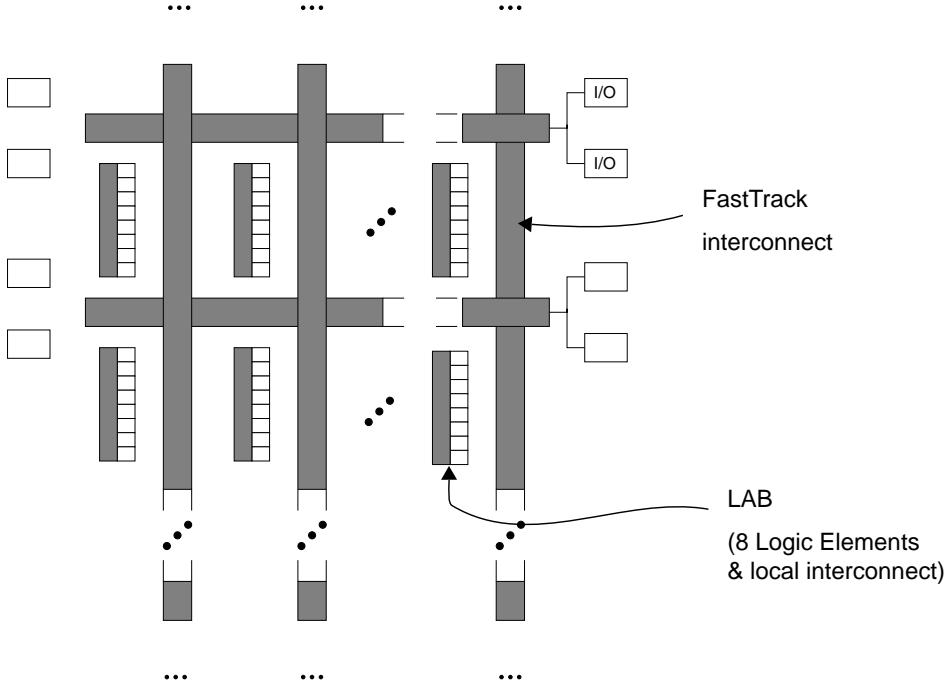
\includegraphics[width=0.5\textwidth]{img1/FLEX800.jpeg}
\textbf{图12:} \emph{Altera FLEX 8000 FPGA 架构。}
\end{frame}

\begin{frame}{\textbf{XADC 模块}}
\begin{itemize}
\tightlist
\item
    模拟信号可以通过采样和量化后被数字系统处理,执行这些操作的模块称为模数转换器(ADC)。由于数字系统的最新进展需要处理模拟信号,Artix-7
    FPGA 专门配备了 XADC 模块。
\item
    Artix-7 XC7A35T FPGA 包含一个 XADC 模块,该模块由两个 ADC
    模块组成。每个模块每秒可以采集 100 万个样本(MSPS),每个样本用 12
    位表示。两个 ADC 模块可以同时处理两个不同的模拟信号。
\end{itemize}
\end{frame}

\begin{frame}{\textbf{高速串行 I/O 收发器}}
\begin{itemize}
\item
    高速串行 I/O
    收发器(HSSIOs)是专门用于传输和接收串行数据的电路。这些收发器是进行速度约为每秒千兆比特(Gb/s)数据传输的必备组件。
\item
    PCIe(外围组件互连高速)是一种高速串行连接总线标准。Artix-7 XC7A35T
    FPGA 包含一个用于 PCIe 接口的集成模块。
\end{itemize}
\end{frame}

\begin{frame}
\begin{itemize}
\tightlist
\item
    \textbf{FLEX 8000 架构}:

    \begin{itemize}
    \tightlist
    \item
    如图13所示,FLEX 8000 的基本逻辑块称为\textbf{逻辑元素(Logic
    Element, LE)},包含一个 4 输入
    LUT、一个触发器以及用于算术电路的特殊进位电路(类似于 Xilinx
    XC4000)。
    \item
    LE 还包括级联电路,可高效实现宽与函数。
    \item
    \textbf{LE 细节}: 如图21所示。
    \end{itemize}
\end{itemize}

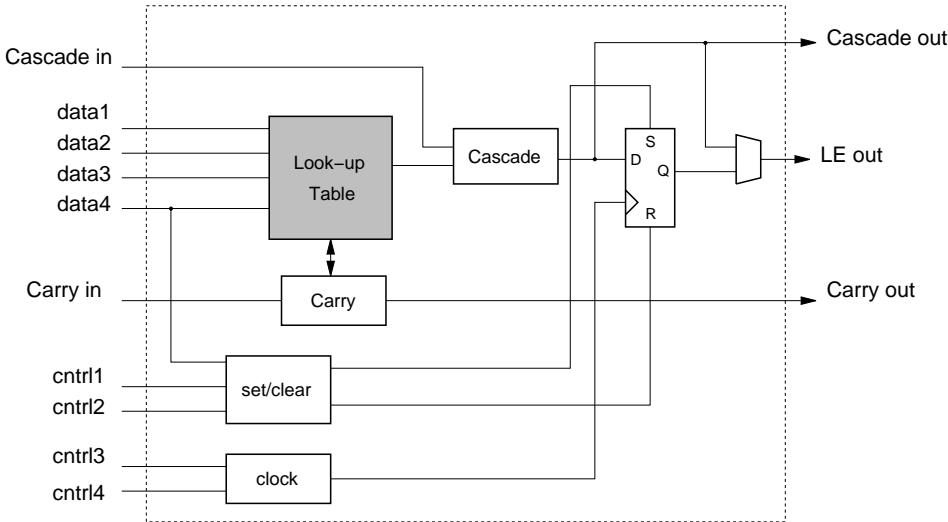
\includegraphics[keepaspectratio]{img1/FLEX800LE.jpeg}
\textbf{图13:} \emph{Altera FLEX 8000 逻辑单元(LE)。}
\end{frame}

\begin{frame}
\begin{itemize}
\tightlist
\item
    \textbf{逻辑阵列块(LAB)}:

    \begin{itemize}
    \tightlist
    \item
    LE 被分组为 8 个一组的\textbf{逻辑阵列块(Logic Array Blocks,
    LABs)},这个概念借用了 Altera 的 CPLD。
    \item
    如图14所示,每个 LAB 包含本地互连,每条本地线可以连接同一 LAB
    内的任何 LE。
    \item
    本地互连还连接到 FLEX 8000 的\textbf{全局互连(FastTrack)}。
    \item
    \textbf{FastTrack}: 类似于 Xilinx 的长线,每条 FastTrack
    线延伸整个芯片的宽度或高度。
    \item
    \textbf{特点}: FLEX 8000 只有长线,这使得 CAD
    工具能够自动配置,且互连延迟比使用许多小段线的 FPGA 更可预测。
    \end{itemize}
\end{itemize}

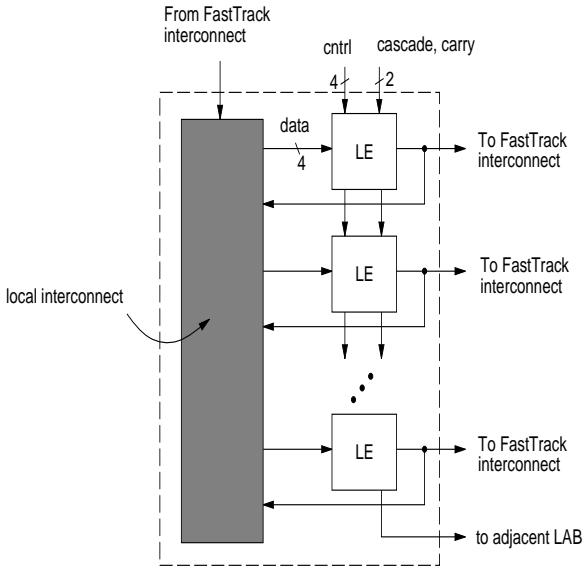
\includegraphics[keepaspectratio]{img1/FLEX800LAB.jpeg}
\textbf{图14:} \emph{Altera FLEX 8000 逻辑阵列块(LAB)。}
\end{frame}

\begin{frame}
\begin{itemize}
\tightlist
\item
    \textbf{FLEX 10000 系列}:

    \begin{itemize}
    \tightlist
    \item
    FLEX 10000 是对 FLEX 8000 架构的扩展,增加了可变大小的 SRAM
    块,称为\textbf{嵌入式阵列块(Embedded Array Blocks, EABs)}。
    \item
    \textbf{EAB 功能}:

    \begin{itemize}
    \tightlist
    \item
        可以配置为具有可变宽高比的 SRAM 块:256 x 8、512 x 4、1K x 2 或 2K
        x 1。
    \item
        也可以配置为实现复杂逻辑电路(如乘法器),作为大型多输出查找表使用。
    \end{itemize}
    \item
    \textbf{CAD 工具支持}: Altera 提供了多个宏函数,用于在 EAB
    中实现有用的逻辑电路。
    \item
    \textbf{逻辑容量}: 目前 FPGA 中最高,但难以提供准确数字。
    \end{itemize}
\end{itemize}

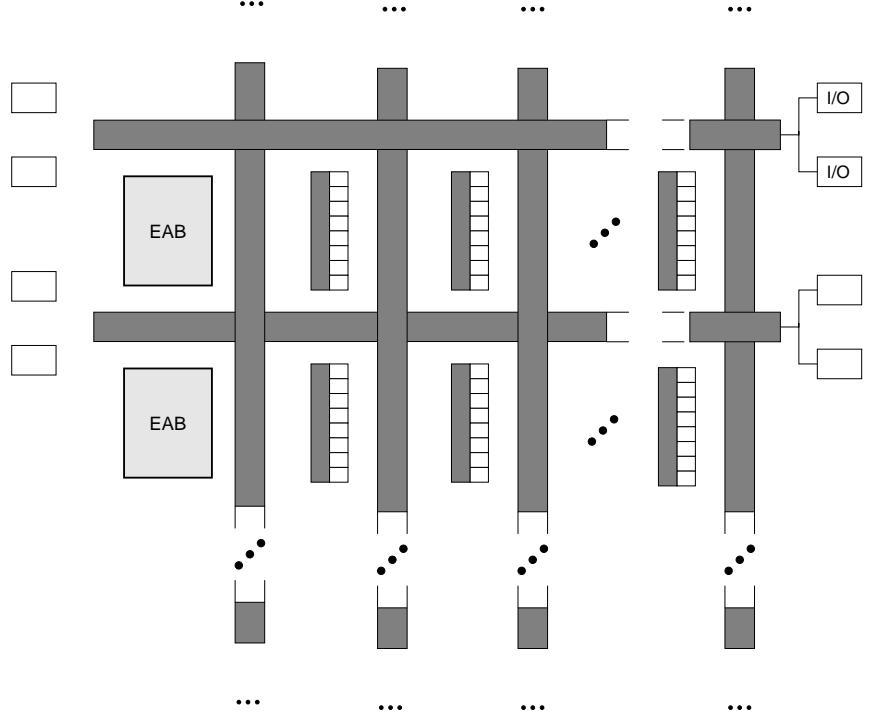
\includegraphics[keepaspectratio]{img1/FLEX10K.jpeg}
\textbf{图15:} \emph{Altera FLEX 10K FPGA 架构。}
\end{frame}

\begin{frame}
\begin{block}{\textbf{FPGA 的应用}}
\phantomsection\label{fpga-ux7684ux5e94ux7528}
\begin{itemize}
\tightlist
\item
    \textbf{概述}:

    \begin{itemize}
    \tightlist
    \item
    FPGA
    在过去十年中迅速获得认可并快速增长,因为它们可以应用于非常广泛的应用领域。
    \item
    \textbf{典型应用}:

    \begin{itemize}
    \tightlist
    \item
        随机逻辑。
    \item
        集成多个 SPLD。
    \item
        设备控制器。
    \item
        通信编码和滤波。
    \item
        包含 SRAM 块的中小型系统。
    \end{itemize}
    \end{itemize}
\item
    \textbf{设计原型与硬件仿真}:

    \begin{itemize}
    \tightlist
    \item
    \textbf{设计原型}: 用于在门阵列中实现的设计原型。

    \begin{itemize}
    \tightlist
    \item
        可能仅需要一个大型 FPGA(容量相当于一个小型门阵列)。
    \end{itemize}
    \item
    \textbf{硬件仿真}: 仿真整个大型硬件系统。

    \begin{itemize}
    \tightlist
    \item
        涉及通过某种互连连接的多个 FPGA。
    \item
        例如,QuickTurn 等公司开发了包含多个 FPGA
        和必要软件的产品,用于电路的分区和映射。
    \end{itemize}
    \end{itemize}
\end{itemize}
\end{block}
\end{frame}

\begin{frame}
\begin{itemize}
\tightlist
\item
    \textbf{定制计算}:

    \begin{itemize}
    \tightlist
    \item
    一个新兴且前景广阔的应用领域是使用 FPGA 作为定制计算机。

    \begin{itemize}
    \tightlist
    \item
        利用可编程部分``执行''软件,而不是将软件编译为在常规 CPU 上执行。
    \item
        相关资源:IEEE 举办的 FPGA-Based Custom Computing Workshop
        (FCCM)。
    \end{itemize}
    \end{itemize}
\item
    \textbf{设计与性能}:

    \begin{itemize}
    \tightlist
    \item
    \textbf{CPLD 映射}: 设计通常自然地映射到类似 SPLD
    的块,性能更可预测。
    \item
    \textbf{FPGA 映射}: 设计被分解为逻辑块大小的部分,并分布在 FPGA
    的区域中。

    \begin{itemize}
    \tightlist
    \item
        由于 FPGA 的互连结构,这些逻辑块之间的连接可能引入各种延迟。
    \item
        因此,FPGA 的性能更多地取决于 CAD 工具如何将电路映射到芯片中。
    \end{itemize}
    \end{itemize}
\end{itemize}
\end{frame}

\begin{frame}
\begin{block}{\textbf{基于 FPGA 的数字系统设计哲学}}
\phantomsection\label{ux57faux4e8e-fpga-ux7684ux6570ux5b57ux7cfbux7edfux8bbeux8ba1ux54f2ux5b66}
\begin{itemize}
\tightlist
\item
    数字系统可以通过不同的设计策略和资源实现。本节讨论使用 FPGA
    进行数字系统设计的哲学,强调如何有效地使用 FPGA。
\end{itemize}
\end{block}

\begin{block}{\textbf{使用 FPGA 时的思考方式}}
\phantomsection\label{ux4f7fux7528-fpga-ux65f6ux7684ux601dux8003ux65b9ux5f0f}
\begin{itemize}
\tightlist
\item
    \textbf{设计自由}: 使用 FPGA
    设计数字系统时,用户可以自由选择设计方法,同一个数字系统可以通过多种方式实现,设计师有责任选择最适合的设计风格。
\item
    \textbf{无预定义模块}: FPGA
    设计开始时没有预定义的模块,设计师需要使用强大的资源来构建所需的模块,因此需要扎实的数字逻辑知识。FPGA
    厂商也提供 IP 模块以简化设计。
\item
    \textbf{硬件描述语言(HDL)}: FPGA
    设计使用硬件描述语言(HDL),而不是传统的顺序编程语言。设计应基于块级并行实现,以获得最佳性能。
\item
    \textbf{可重构性}: FPGA
    可以在初始设计完成后重新配置,用户可以利用这一特性在设计和嵌入设备后改进和修改设计。
\end{itemize}
\end{block}

\begin{block}{\textbf{FPGA 的优缺点}}
\phantomsection\label{fpga-ux7684ux4f18ux7f3aux70b9}
\begin{itemize}
\tightlist
\item
    \textbf{离散元件}:
    离散元件设计需要物理空间和复杂的布线,一旦实现后设计就无法更改。FPGA
    提供了更紧凑的解决方案,且设计可以重新配置。
\item
    \textbf{ASIC}: ASIC
    克服了空间和布线问题,且在大规模生产时成本较低。然而,ASIC
    设计一旦完成就无法更改,且制造时间较长。FPGA
    在原型设计和验证方面具有优势。
\item
    \textbf{微控制器}: 微控制器和 FPGA
    都具有可重构性和紧凑性,但微控制器的指令集限制了其灵活性,且功率消耗较高。FPGA
    具有并行实现能力,操作速度更快,且可以在 FPGA 上实现微控制器。
\end{itemize}
\end{block}

\begin{block}{\textbf{FPGA 的用途}}
\phantomsection\label{fpga-ux7684ux7528ux9014}
FPGA 可以用于几乎所有需要数字系统的领域。为了激励读者并说明学习基于 FPGA
的数字设计的重要性,以下列出 FPGA
的潜在应用领域:航空航天、汽车、广播、消费电子、国防、高性能计算、工业应用、医疗应用以及有线和无线通信。这些并非
FPGA 的唯一应用领域,新的应用可能会随着时间的推移而出现。
\end{block}
\end{frame}

\begin{frame}{FPGA与CPLD的主要区别有}
\phantomsection\label{fpgaux4e0ecpldux7684ux4e3bux8981ux533aux522bux6709}
\begin{enumerate}
\tightlist
\item
    \textbf{架构差异}

    \begin{itemize}
    \tightlist
    \item
    FPGA 采用细粒度结构(LUT + 分布式寄存器),适合复杂时序逻辑。\\
    \item
    CPLD 采用粗粒度结构(乘积项 + 集中式宏单元),适合组合逻辑。
    \end{itemize}
\item
    \textbf{资源规模}

    \begin{itemize}
    \tightlist
    \item
    FPGA 逻辑单元数量多,集成RAM、DSP等模块。\\
    \item
    CPLD 逻辑资源较少,无专用硬件模块。
    \end{itemize}
\item
    \textbf{时序特性}

    \begin{itemize}
    \tightlist
    \item
    FPGA 时序优化依赖工具,延迟不可预测。\\
    \item
    CPLD 时序固定,适合确定性控制。
    \end{itemize}
\item
    \textbf{适用场景}

    \begin{itemize}
    \tightlist
    \item
    FPGA:视频处理、通信协议、AI加速等。\\
    \item
    CPLD:电源管理、接口转换、简单状态机。
    \end{itemize}
\end{enumerate}
\end{frame}

\begin{frame}
\begin{block}{选型建议}
\phantomsection\label{ux9009ux578bux5efaux8bae}
\begin{itemize}
\tightlist
\item
    \textbf{选择
    FPGA}:需要高性能、高灵活性、支持复杂算法或大规模并行处理。\\
\item
    \textbf{选择 CPLD}:要求低功耗、快速启动、确定性延迟和小型逻辑控制。
\end{itemize}
\end{block}

\begin{block}{\textbf{习题}}
\phantomsection\label{ux4e60ux9898}
\begin{itemize}
\tightlist
\item
    \textbf{1} 除了 OR 和 AND 逻辑门外,还有 NOR(NOT-OR)和
    NAND(NOT-AND)门。请使用基本逻辑门结构来构建它们。
\item
    \textbf{2} 在某些应用中还会使用 XOR 门,请使用 OR 和 AND
    逻辑门构建该门。
\item
    \textbf{3} FPGA 并非实现数字系统的唯一设备,请研究过去开发的类似设备。
\item
    \textbf{4} Artix-7 FPGA 是我们在本书中考虑的系列,但 Xilinx 还有其他
    FPGA 系列,请选择两个系列并将其属性与 Artix-7 FPGA 进行比较。
\item
    \textbf{5} Xilinx 并非市场上唯一的 FPGA 生产商,请研究其他生产商。

    \begin{itemize}
    \tightlist
    \item
    \begin{enumerate}
    [a.]
    \tightlist
    \item
        对 FPGA 开发商的市场份额进行评论。
    \end{enumerate}
    \item
    \begin{enumerate}
    [a.]
    \setcounter{enumi}{1}
    \tightlist
    \item
        如果可能,比较不同生产商开发的 FPGA 的通用属性。
    \end{enumerate}
    \end{itemize}
\item
    \textbf{6} 微控制器和 FPGA 的主要区别是什么?
\end{itemize}
\end{block}
\end{frame}
